The approach adopted for video subtitling, as illustrated in Figure~\ref{process}, follows three steps: preparation, annotation and presentation. This is a hybrid approach in which the Owner performs the initial configuration of the project. The Crowd provides suggestions for each of the speeches in the video, and the filtering and aggregation activities are performed by automatic methods.

\begin{figure}[H]
	\centerline{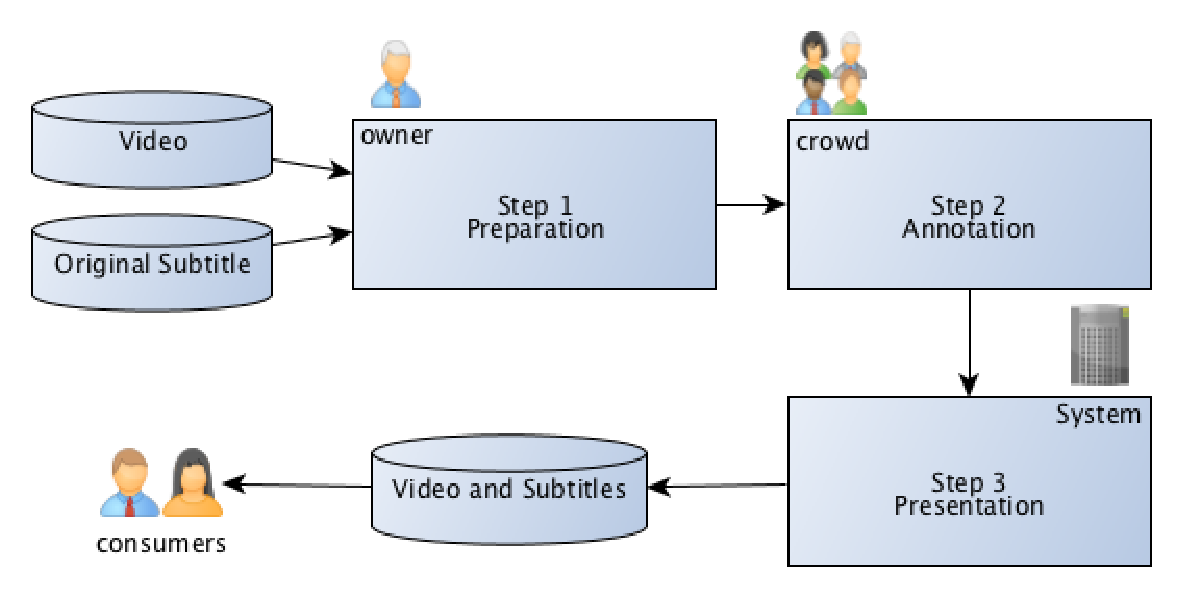
\includegraphics[scale=0.4] {figure/process-workflow}}
	\caption{Process workflow}
	\label{process}
\end{figure}

\subsection{Step 1 - Preparation}
The preparation step is where the video segments that are sent to the workers in each job are defined. The strategy chosen to determine these segments was to process the original video caption file, in the native language, and send in each job a video segment equivalent to a speech contained in it. This process can be seen in Figure~\ref{preparation}.


\begin{figure}[H]
	\centerline{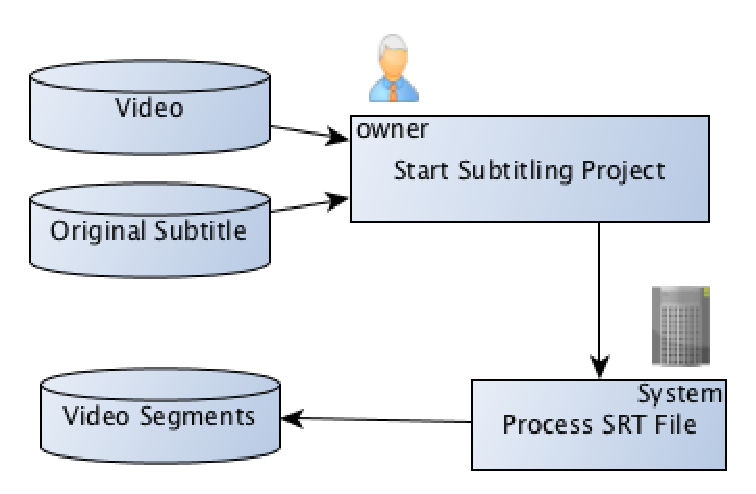
\includegraphics[scale=0.4] {figure/preparation-workflow}}
	\caption{Step 1 workflow}
	\label{preparation}
\end{figure}

\subsection{Step 2 - Annotation}

\begin{figure}[H]
	\centerline{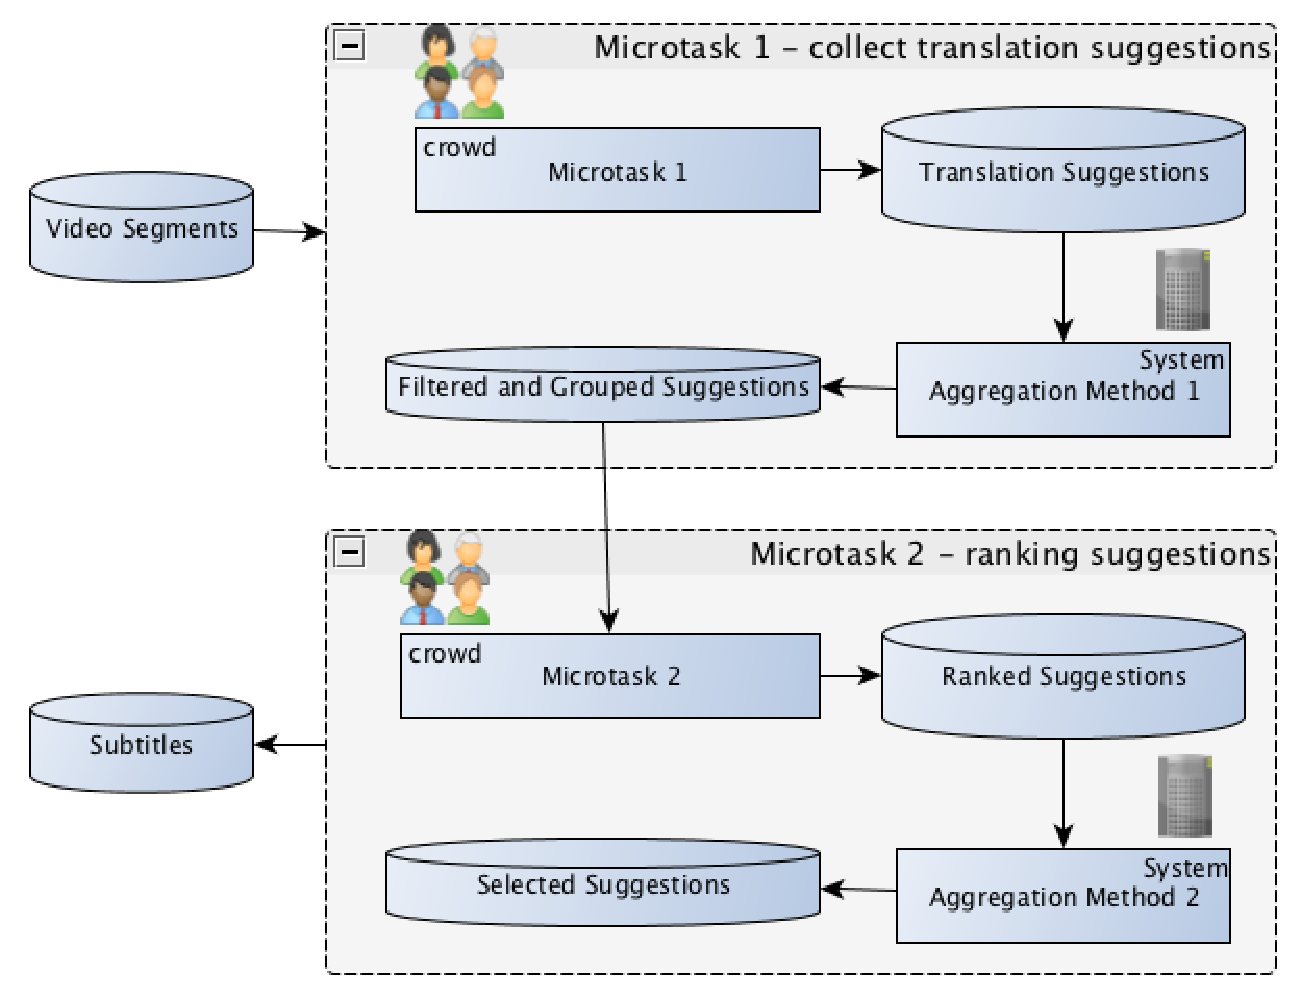
\includegraphics[scale=0.4] {figure/annotation-workflow}}
	\caption{Step 2 workflow}
	\label{annotation}
\end{figure}

\subsection{Step 3 - Presentation}

\begin{figure}[H]
	\centerline{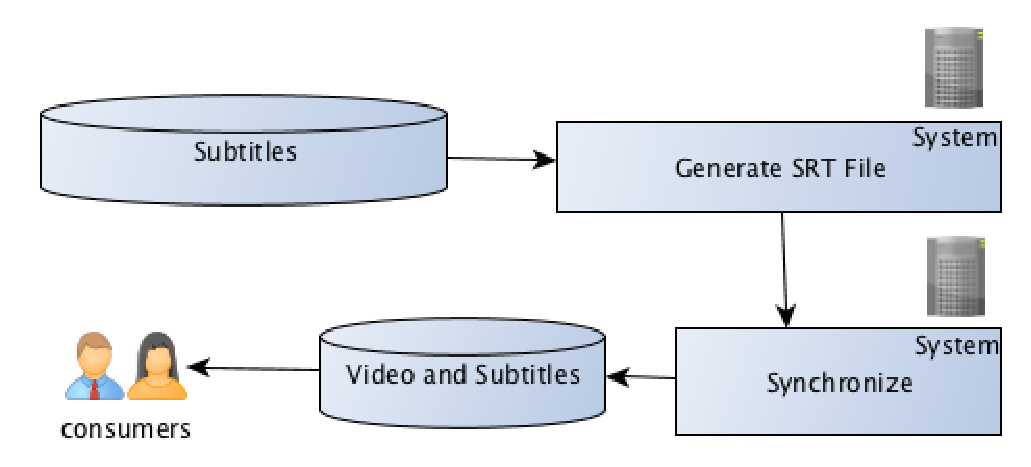
\includegraphics[scale=0.4] {figure/presentation-workflow}}
	\caption{Step 3 workflow}
	\label{presentation}
\end{figure}